\documentclass[]{beamer}
% Class options include: notes, notesonly, handout, trans,
%                        hidesubsections, shadesubsections,
%                        inrow, blue, red, grey, brown

% Theme for beamer presentation.
\usepackage{beamerthemesplit} 
\usepackage{tabularx}
\makeatletter
\def\hlinewd#1{%
\noalign{\ifnum0=`}\fi\hrule \@height #1 %
\futurelet\reserved@a\@xhline}
\makeatother

% Other themes include: beamerthemebars, beamerthemelined, 
%                       beamerthemetree, beamerthemetreebars  
\newcommand{\tab}{\hspace*{2em}}
\newcommand*\oldmacro{}%
\let\oldmacro\insertshorttitle%
\renewcommand*\insertshorttitle{%
  \oldmacro\hfill%
  \insertframenumber\,/\,\inserttotalframenumber}
\title{Malware Reverse Engineering Basic Knowledge}    % Enter your title between curly braces
\author{Andrea Mambretti (mambro007@gmail.com)}        % Enter your name between curly braces
\institute{Politecnico di Milano}      % Enter your institute name between curly braces
\date{\today}                    % Enter the date or \today between curly braces

\begin{document}

% Creates title page of slide show using above information
\begin{frame}
  \titlepage
\end{frame}
\note{Talk for 50 minutes} % Add notes to yourself that will be displayed when
                           % typeset with the notes or notesonly class options

\section[Outline]{}

% Creates table of contents slide incorporating
% all \section and \subsection commands
\begin{frame}
  \tableofcontents
\end{frame}
\section {Crash course on Assembly Language }
	\subsection{An overview on the common 32-bit Inter Architecture (IA)}
		\begin{frame}
			\frametitle{(1) How is the IA made?}
			\begin{itemize}
				\item{ EAX,EBX,ECX,EDX,ESI,EDI,EBP,EIP and ESP }
			\end{itemize}
		\end{frame}
		\begin{frame}
			\frametitle{(2) How is the IA made?}
					\begin{figure}
						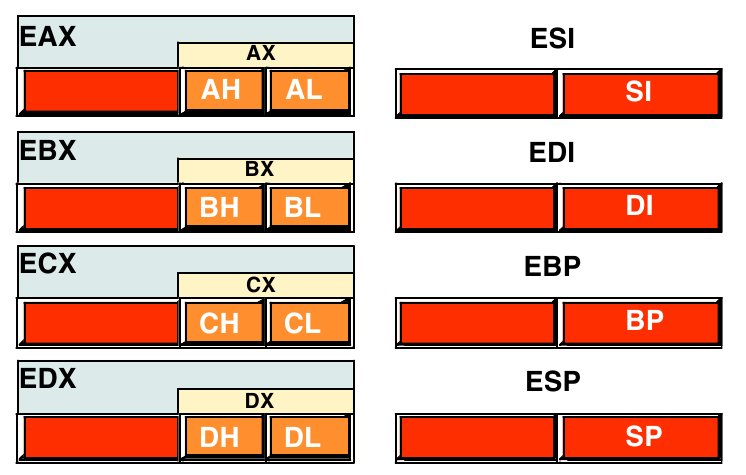
\includegraphics[height=1.6in]{images/registers.jpeg}
						\label{Registers Division}
					\end{figure}
		\end{frame}
		\begin{frame}
			\frametitle{(1) What about EFLAGS?}
			\begin{figure}
				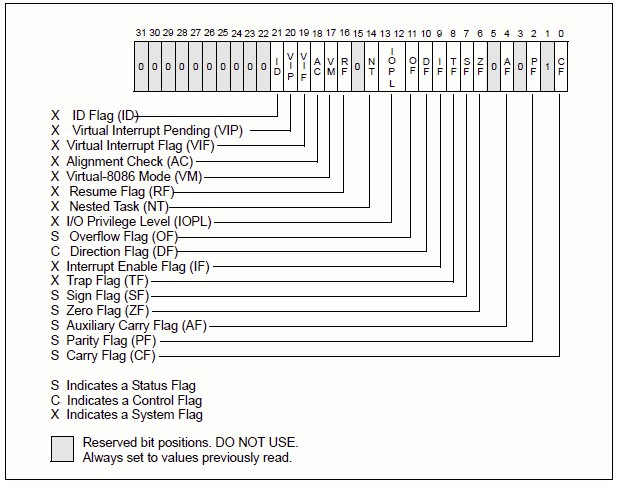
\includegraphics[height=2.5in]{images/eflags.jpeg}
				\label{Eflags idea}
			\end{figure}
		\end{frame}
		\begin{frame}
			\frametitle{(2) What about EFLAGS?}
			\begin{itemize}
				\item{Overflow, Direction, Interrupt Disable, Sign, Zero, Auxiliary Carry, Parity and Carry Flags}
				\item{They are VERY important for the control flow of the program }				
			\end{itemize}
		\end{frame}
	\subsection{Syntaxes overview}
		\begin{frame}
			\frametitle{Syntax}
			\begin{itemize}
				\item{In the assembly world we can find two main syntax the AT\&T and the Intel}
				\item{AT\&T is used by all the UNIX program (gdb)}
				\item{Intel syntax is used by Microsoft program (IDApro and others)}
			\end{itemize}
		\end{frame}
		\begin{frame}
			\frametitle{(1) Differences in the notation}
			\begin{itemize}
				\item{Consider the following operation:\newline\centerline{"move the value 0 to EAX"}}
				\item{AT\&T: \centerline{ mov \$0x0,\%eax} }
				\item{Intel: \centerline{ mov eax, 0h}}
			\end{itemize}
		\end{frame}
		\begin{frame}
			\frametitle{(2) Differences in the notation}
			\begin{itemize}
				\item{Consider this other operation:\newline\centerline {"move the value 0 to the address contained in EBX+4"}}
				\item{AT\&T: \centerline{ mov \$0x0,0x4(\%ebx)}}
				\item{Intel: \centerline{ mov [ebx+4h],0h }}
			\end{itemize}
		\end{frame}
	\subsection{Let's look to the basic instructions}
		\begin{frame}
			\frametitle{(1) Basic Instructions overview}
				\begin{itemize}
					\item{Every processor has a very huge number of instructions to execute (see Intel Manual\footnote{\url{http://www.intel.com/content/www/us/en/processors/architectures-software-developer-manuals.html}})}
					\item{A subset of the whole instructions set is usually dipendent by the considered processor. We will focus on the \underline{other} subset of instructions}
					\item{We will use the Intel syntax to see them because is the same syntax used in IDApro by default}
				\end{itemize}
		\end{frame}
		\begin{frame}
			\frametitle{(2) Basic Instruction MOV}
				\begin{itemize}
					\item{ General: MOV \underline{\textbf{destination}}, \underline{\textbf{source}}}
					\newline		
					\item{	\textbf{source} can be an immediate, a register, a memory location}
					\newline
					\item{	\textbf{destination} can be either a register  or a memory location}
					\newline
					\item{	NB: Every combination is possible except memloc to memloc!!!}
				\end{itemize}
		\end{frame}
		\begin{frame}
			\frametitle{(3) Basic Instruction ADD}
				\begin{itemize}
					\item{General: ADD \underline{\textbf{destination}}, \underline{\textbf{source}}}
					\newline
					\item{\textbf{source} can be an immediate, a register, a memory location}
					\newline
					\item{\textbf{destination} can be either a register or a memory location}
					\newline
					\item{NB: The destination register has to be as big as at least the source or greater }
				\end{itemize}
		\end{frame}
		\begin{frame}
			\frametitle{(4) Basic Instruction SUB}
				\begin{itemize}
					\item{General: SUB \underline{\textbf{destination}}, \underline{\textbf{source}}}
					\newline
					\item{\textbf{source} can be an immediate, a register, a memory location}
					\newline
					\item{\textbf{destination} can be either a register or a memory location}
					\newline
					\item{NB: The destination register has to be as big as at least the source or greater }
				\end{itemize}
		\end{frame}
		\begin{frame}
			\frametitle{(5) Basic Instruction MUL}
			\begin{itemize}
					\item{General: MUL \underline{\textbf{Operand}}}
					\newline
					\item{\textbf{Operand} can be an immediate, a register, a memory location}
					\begin{table}[h]
						\begin{tabular}{|c!{\vrule width 1pt}c|c|c| }
							\hline
							 & 1 byte & 2 bytes& 4 bytes\\	\hlinewd{1.3pt}
							Other Operand& AX     & DX:AX   & EDX:EAX\\	\hline
							Higher Part of result stored in: & AH & DX & EDX\\		\hline
							Lower Part of result  stored in:  & AL & AX & EAX\\
							\hline
						\end{tabular}
					\end{table}
			\end{itemize}
		\end{frame}
		\begin{frame}
			\frametitle{(6) Basic Instruction DIV}
			\begin{itemize}
					\item{General: DIV \underline{\textbf{Operand}}}
					\newline
					\item{\textbf{Operand} can be an immediate, a register, a memory location}
					\begin{table}[h]
						\begin{tabular}{|c!{\vrule width 1pt}c|c|c| }
							\hline
							 & 1 byte & 2 bytes & 4 bytes\\	\hlinewd{1.3pt}
							Dividend     & AX     & DX:AX   & EDX:EAX\\	\hline
							Remainder stored in: & AH & DX & EDX\\		\hline
							Quotient stored in:  & AL & AX & EAX\\
							\hline
						\end{tabular}
					\end{table}
			\end{itemize}
		\end{frame}


		\begin{frame}
			\frametitle{(7) Basic Instruction CMP}
				\begin{itemize}
				\item{General: CMP \underline{\textbf{Operand\_1}}, \underline{\textbf{Operand\_2}}\\
					\textbf{Operand\_1} can be an immediate, a register, a memory location\\
					\textbf{Operand\_2} can be either a register or a memory location\\}
		\end{frame}

		
		\begin{frame}
			\frametitle{(8) Basic Instruction JMP}
			\begin{itemize}
				\item{With this instruction we can add a value from \textbf{source}  to the destination operand and put the new value inside the destination}
				\item{General: DIV \underline{\textbf{operand}}\\
					\textbf{operand} can be an immediate, a register, a memory location\\
					NB: The destination register has to be as big as at least the source or greater} 
				\item{Examples}
					\begin{columns}
						\begin{column}[left]{1.7in}
							\begin{itemize}
								\item{ADD esp, 44h}
								\item{ADD eax, ebx}
							\end{itemize}
						\end{column}
						\begin{column}[center]{1.5in}
							\begin{itemize}
								\item{ADD al, dh}
								\item{ADD edx, cx}
							\end{itemize}
						\end{column}
						\begin{column}[right]{2in}
							\begin{itemize}
								\item{ADD [eax],[ecx] NO!!!}
								\item{ADD [eax],1h}
							\end{itemize}
						\end{column}
					\end{columns}
			\end{itemize}
		\end{frame}
	\subsection{...givi}


\section {Overview on the Analysis Techniques }
	\subsection{Basic static Analysis}
		\begin{frame}
			\frametitle{What is Basic Static Analysis?}
			
			\begin{itemize}
				\item {B.S.A. consists in a very simple set of operation that can allow a malware analyst to get usefull information about a certain binary file}
				\item {B.S.A. tools can give us infomation about:}
				\begin{itemize}
					\item{\textbf{Antivirus Scanning}: tell us if it is an already known malware or not and if yes which kind (ex www.virustotal.com) }
					\item{\textbf{Hashing}: tell if a certain file has been corrupted or not}
					\item{\textbf{Strings}: give us all the strings defined as costant in the program that can be usefull to undestand what that file does}
					\item{\textbf{Recognizers Packing and Obfuscation}: if the file uses some type of packing (ex: upx) or obfuscation to avoid recognition} 
					\item{\textbf{Header Analysis}: Looking inside the header give us information about import and export function, when it's compiled, if it's packet, if there's some extra segment and other stuff }
				\end{itemize}
			\end{itemize}
		\end{frame}
		\begin{frame}
			\frametitle{When is it necessary?}
			\begin{itemize}
				\item {If someone is really paranoic the answer is every time before launch  an application }
				\item {for all the others when something of suspicious is detected during the previous execution}
				\item {after this phase a human analyzer knows if it is needed to procede with other analysis such as dynamic and advaced static analysis}
			\end{itemize}	
		\end{frame}

	\subsection{Dynamic Analysis}
		\begin{frame}
			\frametitle{What is Dynamic Analysis?}
			\begin{itemize}
				\item {D.A. consists in  looking the behaviour of a malware running it and loggin every change and action done in the system}
				\item {of course is not always possible use this technique because a specific malware can damage the system and makes the information unreachable}
				\item {so what can we do to avoid it?}
			\end{itemize}
		\end{frame}
		\begin{frame}
			\frametitle{Possible Solution: Virtual Machine}
			\begin{itemize}
				\item {Using Virtual Machine we can set a perfect enviroment for our malware (fake a whole network of hosts,logger etc. )}
				\item {We can check out of box what happens inside (system call, network operation etc.).\newline
					if something goes wrong we can, using snapshots, rollback the machine state to a sane position					    }
				\item {Possible sequence of operation:}
					\begin{itemize}
						\item{Start with a clean snapshot with no malware running on it}
						\item{Trasfer the malware to the virtual machine}
						\item{Conduct your analysis on the virtual machine}
						\item{Take your notes, screenshots, and data from the virtual machine and transfer it to the physical machine}
						\item{Revert the virtual machine to the clean snapshot}			
					\end{itemize}	
			\end{itemize}
		\end{frame}
		\begin{frame}
			\frametitle{Existing VM}
			\begin{block}{VM}
				Someone of them are already prepared to Malware Analysis	
				\begin{itemize}
					\item{VMware}
					\item{VirtualBox}
					\item{Qemu}
					\item{Cuckoo}
					\item{Anubis}
					\item{Andrubis}
					\item{A ton of others}
				\end{itemize}
			\end{block}
		\end{frame}
		\begin{frame}
			\frametitle{Problems and Solution}
			\begin{block}{Problems}
				\begin{itemize}
					\item{It's prooved Today's Malware can avoid the dynamic analysis. They recognize all the well-know VB and they change their behavior when are runned in }
					\item{The worst scenario happens when specific malware are done to exploit vulnerabilities inside VM to own the whole machine where the VB is running}
				\end{itemize}
			\end{block}
			\begin{block}{Solution}
				\begin{itemize}
					\item{One of the possible solution to understand if the malware has behaved not in his standard way and which are his possibility is to see the code more deeply with the Advanced Static Analysis (aka Reverse Engineering) }
				\end{itemize}
			\end{block}
		\end{frame}

	\subsection{Advanced Static Analysis}
		\begin{frame}
			\frametitle{What is Reverse Engineering in General?}
			
			\begin{block}{Definition}
				\begin{itemize}
					\item{Reverse engineering is taking apart an object to see how it works in order to duplicate or enhance the object. The practice, taken from older industries, is now frequently used on computer hardware and software.}
					\item{Reverse engineering is usually conducted to obtain missin knowledge, ideas, adn design philosophy when such information is unavailable}
				\end{itemize}
			\end{block}
		\end{frame}	
		\begin{frame}	
			\frametitle{What is Software reverse engineering?}
			\begin{block}{Definition}
				\begin{itemize}
					\item{Software reverse engineering involves reversing a program's machine code (the string of 0s and 1s that are sent to the logic processor) back into the assembly language (x86, x86-64, ARM so on and so forth) }
					\item{Software reverse engineering requires a combination of skills and a thorough undestanding of computers and software development, but like most worthwhile subjects, the only real prerequisite is a strong curiosity and desire to learn. Software reverse engineering integrates several arts: code breaking, puzzle solving, programming, and logical analysis.}
				\end{itemize}
			\end{block}
		\end{frame}
		\begin{frame}
			\frametitle{When do we use it?}
			\begin{itemize}
				\item{Reversing Application}
				\item{Security-Related Reversing}
					\begin{itemize}
						\item{Malicious Software}
						\item{Reversing Cryptographic Algorithms}
						\item{Digital Rights Management}
						\item{Auditing Program Binaries}
					\end{itemize}
				\item{Reversing Software Development}
					\begin{itemize}
						\item{Achieving Interoperability with Proprietary Software}
						\item{Developing Competing Software}
						\item{Evaluating Software Quality and Robustness}
					\end{itemize}
			\end{itemize}			
		\end{frame}
		\begin{frame}
			\frametitle{Background of a good Reverser}
			\begin{itemize}
				\item{Assembly Language}
				\item{Compilers}
				\item{Virtual Machine and Bytecodes (ex Java)}
				\item{Operative Systems}
			\end{itemize}
		\end{frame}
		\begin{frame}
			\frametitle{Tools of a good Reverser}
				\begin{itemize}
					\item{System-Monitoring Tools}
					\item{Disassemblers}
					\item{Debuggers}
					\item{Decompilers}
				\end{itemize}
		\end{frame}
		\begin{frame}
			\frametitle{Some Common Reversing Tools}
			\begin{itemize}
				\item{IDA Pro}
				\item{OllyDbg}
				\item{WinDbg}
				\item{PEBrowse Professional Interactive}
				\item{SoftICE}
			\end{itemize}
		\end{frame}

		\begin{frame}
			\frametitle{Is it Legal?}
			\begin{itemize}
				\item{The Legal debate around reverse engineering has been going on for years}
				\item{1998 -  Digital Millenium Copyright Act}
					\begin{itemize}
						\item{Circumvention of copyright protection systems}
						\item{The development of circumvention technologies}
					\end{itemize}
				\item{Luckily, DMCA makes several exceptions}
					\begin{itemize}
						\item{Interoperability}
						\item{Encryption research}
						\item{Security testing}
						\item{Educational institutions and public libraries}
						\item{Government investigation}
						\item{Regulation}
						\item{Protection of privacy}
					\end{itemize}
			\end{itemize}
		\end{frame}
		\begin{frame}
			\frametitle{Reverse on Malware and Antireversing Techniques}
			Today's malware and commercial program use techniques against Reversing
			\begin{itemize}
				\item{Anti-Disassembly (Linear and Flow Oriented Disassembly)}
					\begin{itemize}
						\item{Jump instructions with the same target}
						\item{Jump instruction with a Costant Condition}
						\item{Impossible disassembly}
					\end{itemize}
				\item{Anti-Debugging}
					\begin{itemize}
						\item{They understand that are executed in a debugger and change their behaviour either crashing itself, the debugger or totally doing other stuff}
					\end{itemize}
				\item{Anti-Virtual Machine Techniques}
				\item{Packers and Unpacking}
			\end{itemize}
		\end{frame}
	 	\begin{frame}
			\frametitle{Conclusion}
			\begin{itemize}
				\item{Software Reverse Engineering is a very powerfull instrument but it requires a lot of lowlevel-knowledge }
				\item{Appling this technique on malware analysis is not optional if we want undestand how the malware works}
				\item{Can be very time consuming and if all the tools used for the analysis are not setted correctly there's no way to reverse the malware }
			\end{itemize}
		\end{frame}
		\begin{frame}
			\frametitle{End}
			\begin{itemize}
				\item{Thanks Folk...Questions?}
				\item{So now one practical example}
			\end{itemize}
		\end{frame}
%\begin{frame}
%  \frametitle{Simple slide with three points shown in succession}   % Insert frame title between curly braces

%  \begin{itemize}
%  \item<1-> Point 1 (Click ``Next Page'' to see Point 2) % Use Next Page to go to Point 2
%  \item<2-> Point 2  % Use Next Page to go to Point 3
%  \item<3-> Point 3
%  \end{itemize}
%\end{frame}
%\note{Speak clearly}  % Add notes to yourself that will be displayed when
                      % typeset with the notes or notesonly class options



%\begin{frame}
 % \frametitle{Slide with two columns: items and a graphic}   % Insert frame title between curly braces
  %\begin{columns}[c]
 % \column{2in}  % slides are 3in high by 5in wide
 % \begin{itemize}
 %\item<1-> First item
 % \item<2-> Second item
 % \item<3-> ...
 % \end{itemize}
 % \column{2in}
 % \framebox{Insert graphic here % e.g. \includegraphics[height=2.65in]{graphic}
 % }
 % \end{columns}
%\end{frame}
%\note{The end}       % Add notes to yourself that will be displayed when
		     % typeset with the notes or notesonly class options

\end{document}
